%-*-texinfo-*-
%This is part of the "UFO:Alien Invasion"-Reference Manuals Tex sources.
%Copyright (C) 2006 Eric Goller.
%Please see licence information at the end of file

%---------------------------------------------------------------------------
%							Version history
%
%  date		/		changes																	/		comment						/	 author
%	06.10.06	/	rev. 0.0.5 (alpha) released											/	complete aspell-check		/	Elbenfreund
%
%---------------------------------------------------------------------------


\documentclass{scrartcl}
\usepackage{anysize,graphicx}
\usepackage[
    pdftex,
    a4paper,
    bookmarks,
    bookmarksopen=true,
    bookmarksnumbered=true,
    colorlinks,
    linkcolor=blue,
    urlcolor=blue
]{hyperref}
\title{UFO: Alien Invasion - Manual [Rev. 0.0.9]}
\author{Eric Goller [elbenfreund (at) gmx (dot) net]}
\date{\today}
%\titlehead{UFO:AI Development-Team and contributing Community}
%\subject{manual}
\publishers{UFO:AI Development-Team and contributing Community: http://ufoai.sf.net}

\begin{document}

Copyright (c)  2006 Eric Goller.\\
Permission is granted to copy, distribute and/or modify this document\\
under the terms of the GNU Free Documentation License, Version 1.2\\
or any later version published by the Free Software Foundation;\\
with no Invariant Sections, no Front-Cover Texts, and no Back-Cover\\
Texts.  A copy of the license is included in the section entitled "GNU\\
Free Documentation License".\\

UFO:AI and its manual are pure free software projects. Nevertheless any pictures, symbols (if any) etc. appearing are subject to the copyright of their respective owners. If you feel that something might conflict with your legal rights please let us know. Otherwise feel free to enjoy free software - free as in freedom ;) 
%to-do: placement in the middle of page

\maketitle
\newpage
%

%---------------------------------------------------------------------------
%							Version history
%
%  date		/		changes																	/		comment						/ author
%	06.10.06	/	rev. 0.0.5 (alpha) released											/	complete aspell-check		/	Elbenfreund
%
%---------------------------------------------------------------------------


Copyright (c)  2006 Eric Goller.
  Permission is granted to copy, distribute and/or modify this document
  under the terms of the GNU Free Documentation License, Version 1.2
  or any later version published by the Free Software Foundation;
  with no Invariant Sections, no Front-Cover Texts, and no Back-Cover
  Texts.  A copy of the license is included in the section entitled "GNU
  Free Documentation License".

\tableofcontents


\subsection{UFO:AI - the beginning}
The original engine development was done as an extreme modification of IDs famous Quake 2 engine by a team around Herby (see credits in the appendix) in \textbf{????}. After \textbf{??} years people lost interest on the project while additionally Herby didn't had the as much time at his hand as in the early days.
To prevent that all the work already invested till that stage (tech demo 2) is lost he took the offer of one of the former contributors (Mattn) to make it open source.  Since those days the source code is hosted by sourceforge.org and given to the community which is asked to use this chance to resurrect one of the most unique and influential games ever. After a short time it became clear that the interest in supporting the development of UFO:AI was unbroken and a bunch of volunteers found together to add their flavour and skill up to what you have in front of you nowadays.

\section{Free games / the community}
This game is brought to you by the UFO:AI Development team and its countless contributors. All of them share at least one thought: to make UFO:AI a great free \footnote{free as in freedom}
 game. Besides detailed legal implications, mentioned in the following section and given in the appendix, most of all this means that every piece of code used to create this game is publicly available. Even more: you are free - even wanted - to change everything you want by yourself whenever you feel you can help making UFO:AI a better way to waste time. This may start with typos or end with complete mods or patches - it's up to you. With UFO:AI being an open-source development by a bunch of non profit orientated people this does also mean there is no big company in the back to pay for extensive testing, balancing or hardwarechecking. So whenever you encounter a bug, a hardware incompatibility or any other problem it would be a fair gesture to give something back to the community - even a carefully filled out bugreport helps a lot. So we hope to do our little share to promote free software and build up a productive open-source gaming community. And no matter what kind of skills you call your own, if you are a coder, 2D or 3D artist, map-designer, even film-script writer, musician, concept-art designer (all of these made UFO:AI what it is today) be assured that there is a project out there waiting for your help - enriching the pool of free software.

\subsection{Contact / Support}
Support, additional information, FAQs and the forum can be found at \url{http://ufoai.sf.net}.
For a release history, latest releases and bugfixes as well as the bug- and featuretracker please see our project page at \url{http://www.sourceforge.org}.
Sourceforge also offers you to take a look at our project page (where you find detailed status reports, contribution- and memberlists). In addition to the forum we also host channel UFO:AI on the freenode IRC network (irc.freenode.org) named UFO:AI. As usual and according to netiquette pleases make sure you try to find solutions for rather trivial problems on your own before asking on the board or on IRC.\\
For interested media we also provide screenshots and offer further support for any planed coverage - feel free to contact us personally by one of the above ways.

\section{Geoscape}

\subsection{Worldmap - an overview} 
Welcome to Geoscape! As said before UFO:AI distincts between two major aspects of the game -- macromanagement and tactical combat. To put it simply, one could say: Combat is where you earn the bucks (and the honour, of course), Geoscape is where you spend them.

Geoscape itself basically consists of two screens. The first one is the world map, which is the first screen you will see right after starting a new campaign. It is used to get the bigger picture of world events as well as coordinating combat missions and intercepting enemy UFOs. The other screen is the base overview, where you improve infrastructure and implement decisions about equipment, research and production. In the following sections we will take a closer look at both of these screens.

The following screenshot shows the uses to which we can put the world map. Observe that it is divided into day and night zones, which influences any combat missions you get into (the day/night borderline changes its shape according to the seasons as the relation earth to sun changes).\\

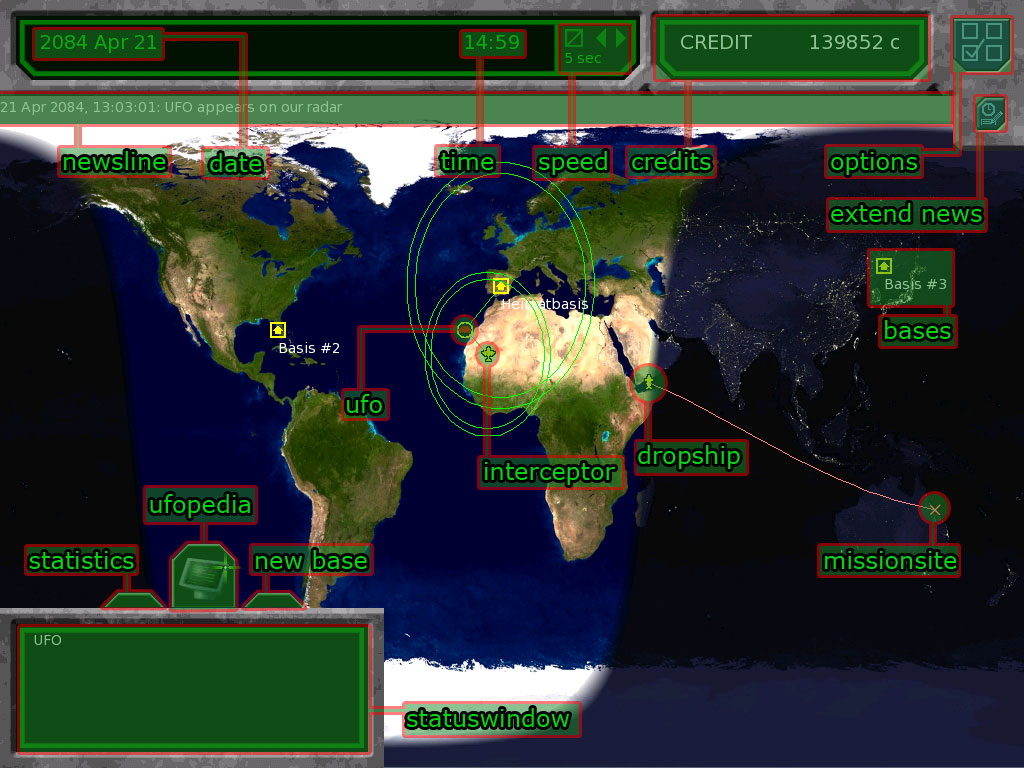
\includegraphics[width=\textwidth]{images/geoscape_final.jpg}

\newpage

\subsubsection{Status Window}
Here some general information(e.g. stats, descriptions) will show up, depending on the context. More detail on each piece of information is given in subsequent sections.
\subsubsection{Statistics}
If you hover over those registers three different buttons will show up. The leftmost leads to some more detailed statistics about your attempt to save the world. In addition to more general information (like missions won/lost etc.) you can also find out about the attitude of all the UN countries paying you. You should be aware that if you fail to protect particular countries from alien invasions (maybe because your infrastructure is not well established in that region) they will cut your resources -- both financial and potential employees.
\subsubsection{Ufopedia}
The middle button is the Ufopedia, a comprehensive collection of useful information about items, technologies, damage types and so on. As your research proceeds Ufopedia grows as well, so make sure you check out the latest information on your enemies every now and then.
\subsubsection{New base}
The rightmost button gives you the chance to establish a new base anywhere on the map, provided it's on land. A new base, once you have built new structures, can give additional radar range, research and production capacities as well as new hangars for your aircraft.  New bases are completely equal to your first in all ways.
\subsubsection{Date}
Gives you the current date, so you know when it's close to pay day. You should also keep an eye on the date, because while you (in principle) have unlimited time to play the game, the aliens get stronger and better equipped as the game proceeds. It is in humanity's best interest if you can catch up with them sooner than later in order to save your beloved homeworld.
\subsubsection{Time and Game Speed}
This is where you can adjust the gamespeed from 5secs (which is in fact pausing the game) all the way through to 1 day steps. Whatever this is set to, while you are in combat time is stopped and it will be all the same when you return from battle.  The game will also automatically pause for certain events like UFO spottings and landings.
\subsubsection{Credits}
Never forget that you can't spend what you don't have.
\subsubsection{Options}
Gets you to the Options-menu where you can load and save your game as well as start a new one.
Through ``exit'' you reach the main menu where you can change game settings and continue your current game (via Single Player $\rightarrow$ Continue)
\subsubsection{News and extended news}
The permanent news line in the upper left always represents the latest news (such as promotions / cashflow / attacks / UFO-sightings) while the extended news button pops up a list of the last 20 new lines. So whenever you notice news, make sure to check the button as well so you don't miss anything. 
\subsubsection{Bases}
The yellow houses represent your bases. Circles around them (popping up later in the game) represent the range of their radars. If you want to ``enter'' a base, just click on its symbol.
\subsubsection{Your dropship}
This is the one that gets your squad to action. Clicking on it once brings up some general data about your ship, like fuel, speed, status and number of assigned soldiers. A second click while it's selected opens a submenu where you may give/change orders, such as sending it back home.
\subsubsection{Your interceptors}
The job of those fast ships is to shoot enemy UFOs down. If your interceptor catches up with a UFA, the dogfight is calculated based on the equipment of both ships; the results are shown on screen. A single click selects the interceptor, while a click on the map will order it to move it there. A second click while the ship is selected brings up a window where you might give it more advanced orders.
\subsubsection{Upcoming missions}
This is where the action waits. Selecting a mission will give you a short description on the status screen while a second one allows you to select a ship to bring in the troops you want.
%-*-texinfo-*-
%This is part of the "UFO:Alien Invasion"-Reference Manuals Tex sources.
%Copyright (C) 2006 Eric Goller.
%See the file ufo-manual_EN.tex for copying conditions.

%---------------------------------------------------------------------------
%							Version history
%
%  date		/		changes																	/		comment						/ author
%	06.10.06	/	rev. 0.0.5 (alpha) released											/	complete aspell-check		/	Elbenfreund
%
%---------------------------------------------------------------------------


\chapter{Tactical combat - Battlescape}

.

\section{Battlescape - an overview}
So this is where all the fun happens ;) It is here that your former choices have to proof their worth as well as you will have to prove your commanding skills.

The goal of every tactical combat is quite simple: kill all those evil aliens with as few civilian (and of cause squad) looses as possible. In order to achieve this you will have to find a good balance between caution and fast proceedings. You don't want to watch all innocents die like flies just because your soldiers are afraid of the enemy.

In the course of the game you will see a wide range of settings and environments, but no matter how bad things may look like, there a some quite powerfull tools at you hand to get rid of them. The main task of the following section is to get familiar with most of them. If you have some experience with (turn-based) tactical combat games you should find some redundant elements - and of cause you will if you ever played any other UFO before. Nevertheless you should take a short overview over the interface so you make sure you don't miss any important feature. To change the view within battlescape you may use either cursor buttons or "WASD". Please be aware that its also possible to change the pitch of the camera. ("R" and "F" by default)

\subsection{Buttons}
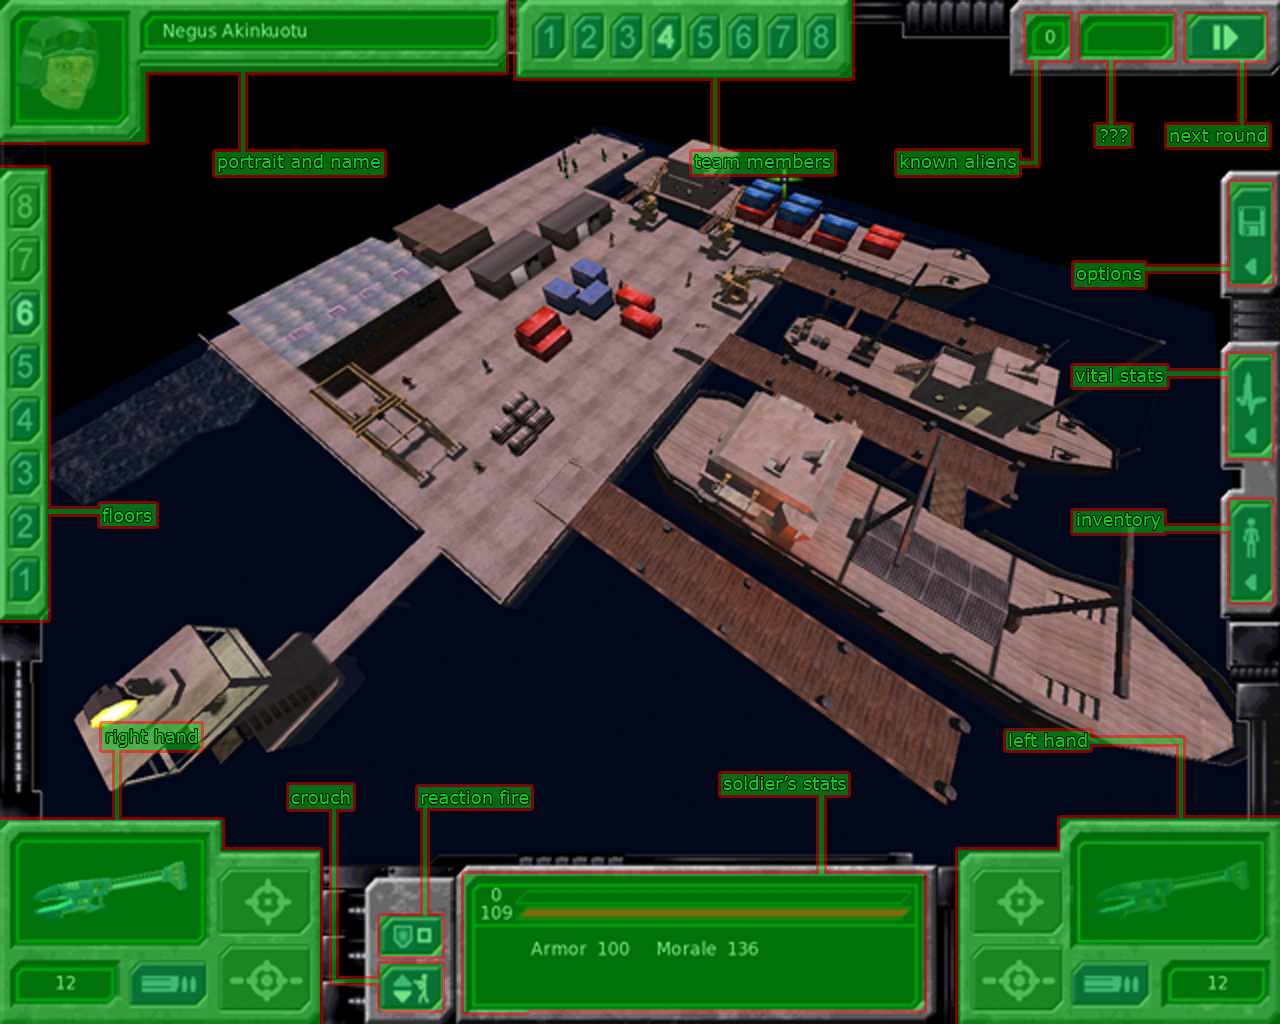
\includegraphics[width=\textwidth]{images/HQ/tactical_overview_finalHQ.jpg}
\subsection{Floors}
Here you can change the "ground-level" or floor shown in the tactical view. Besides its obvious use in order to move you soldiers between different floor-levels it's also helpful to get an general overview. So it's always a smart move to switch between all levels at the beginning of each mission so you won't miss the "hidden" cellar or rooftop.
\subsection{Portrait and name}
This is more for aesthetic reasons, so no big actions are bound to this. (But of cause - as usual- suggestions are welcome)
\subsection{Team-members}
There is where you can switch between you soldiers (alternatively use keybindings: 1 to 8 or just left-click on their model). In case one (or more *G*) of your devoted fighters lost their live fighting the evil his button will become grey.
\subsection{Known aliens}
This states the number of aliens all your squad member have discovered this round. By clicking on it you may switch through all of them.
\subsection{???}
\textbf{I don't have a glue what this is for. Maybe someone wants to give me a hint... ? ;)}
\subsection{next round}
Hmm... so what do you suspect this one does ? Exactly !
\subsection{Options}
Opens the "Options"-menu where you may vary several video/sound-settings as well as aboard or retry current missions. Be aware that it's not possible nor intended to save a ongoing mission.
\subsection{Vital stats}
This is where you find more detailed information about health, moral and psi-power of your soldier.
\subsection{Inventory}
Opens the inventory of the selected soldier. This is where you can change weapons, pick up/drop items or just take a look at your great heroes.
\subsection{Soldiers stats}
This is a summery of all general information you need to use your soldier most efficiently. Its content interacts with your mouse action, but should be quite self-explaining. Not only you will find health and remaining TUs (we will deal with TUs in the following section) here but also it will give you the amount your currently selected shooting-mode will consume as well as some other info's like current armor and moral.
\subsection{Reaction fire}
This button enables "reaction fire", a central concept of every tactical combat. We will deal with it in the following chapter. For now you should just remember that it is here where you turn it on and off.
\subsection{Crouch}
As one might guess, this button will make your soldier kneel down (and by doing so reducing the danger of being hit by enemy fire) or if he already does make him stand up. Please notice that a soldier that kneels down can still move forward as if he would stand upright, but it takes him 1 additional time unit per square to do so.
\subsection{Right/left-hand}
Those two fields are completely identical besides the fact the left hand one is active only if you actually wear two one-handed items/weapons. If you have a two-handed item/weapon equiped the left-hand field will be inactive. Because each of the two fields consist of several important buttons itself we will discuss them a bit more detailed. Please take a look at the following image.
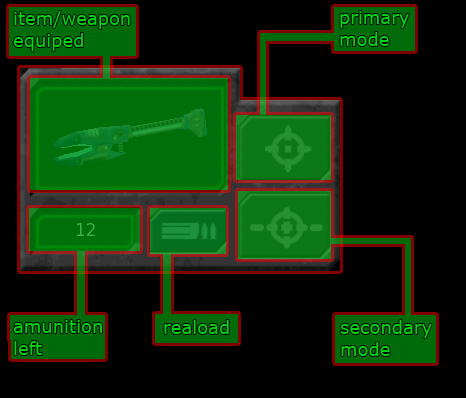
\includegraphics[width=6cm]{images/HQ/weapon_buttons_finalHQ.jpg}
%as float ?!
%transparent background ?! ->going to be re-worked soon
\subsubsection{Item/weapon}
Gives a picture of the currently equiped item/weapon. This turnes red in case you can't use the weapon, for example because you don't know the tech or don't have any ammunition left.
\subsubsection{Primary-mode}
Activates primary-mode for this item. In case of weapons this is usually (but not always!) a fast but less accurate / powerfull shoot. For Details see weapon description.
\subparagraph{Secondary-mode}
Activates secondary-mode for this item. In case of weapons this is usually (but again, not always!) a more TU-consuming but also more accurate / powerfull shoot. Please notice that in case the item supports only one mode (like stun rod) both modes are identical.
\subsubsection{Reload}
Reloads currently equiped weapon, if ammunition is left in the inventory.
\subparagraph{Amunition left}
Shows the ammunition left in your weapon. Please notice that some shooting-modes (also some of the one-shoot ones) require more than one "bullet" here.

\subsection{What to do now ... ?}
%needed ?!

\section{Game-mechanics (Battlescape)}

\subsection{Time-units (TUs)}
As mentioned before every soldier has a certain amount of time units (TUs) which are mainly determined by his "speed" attribute. Every action done by him costs a varying amount of TUs this holds for firing or reloading a weapon as well as walking or re-equipping him in the inventory. The amount of TUs needed for using the primary/secondary mode is given in the status window after selecting one of the two.

\subsection{Movement}
Like firing a weapon, movement also consumes time units. You can make your soldier walk to a spot using your mouse on the tactical view. You will notice that your cursor turns to a green square indicating that this place is reachable with your current amount of TUs or turn blue if it is not (this might be the case due to a lack of TUs or for geographical reasons). If the square is green it will also prompt two numbers of which the first one states the TU-cost of this movement while the second one represents your actual amount of TUs. In case your soldier notices a new enemy or civilian in his line of sight while walking the movement will be interrupted, giving you the chance to adjust your orders according to this new situation.

\subsection{Line of sight}
For obvious reasons you soldiers, in general, can only shoot at what they do see. After finishing an ordered movement your soldier will look in the direction of his last step, which is not very helpful in a lot of situations. To solve this you might make use of the possibility to change your soldiers viewing direction. This can be done in different ways, eg. 3rd-mouse-button / ctrl.-button/ q-button (default-settings). For details please refer to your keybindings. 
\subsection{Shooting-modes}
As we have said before most items, weapons in particular, do have two different action/firing-modes. While the second firing-mode of a sniper rifle is an aimed shot, some assault rifles can start a long fireburst or fire one concentrated and by that devastating single beam. Whatever weapon raises you interest, Ufopedia is your friend. If you look up a certain weapon like that you might be confused, the only information that can be found here is its name and if its a twohanded one or not. What seems rather wired on first sight has a simple reason. As some weapons can be equiped with a wide range of different kinds of ammunition their use and stats also heavily depend on the ammunition loaded. So once you look up the ammunition you want to use you will find all the data and statistics you are looking for - given you have done the required research. Doing so you will find that different firing-modes not only differ by TU needed and damage done but also by weapon skills needed.
\subsection{Chance to hit}



\subsection{Close combat }
An alien is popping up just around the corner and not enough TUs left to fire this Plasma-Blaster in secondary mode while primary-mode offers only indirect fire? Your soldiers being keen on some extra thrill ? You want to capture an living alien for "interrogation"   but all your research department has to offer is a stun rod of which they say it might work - somehow... ? No matter what the reasons may be, there will be a time you will get into close-combat, or it will get to you. While the reason to be that close to an hostile alien might be quite scary, lucky enough the way to use the interface in such a situation is not at all. Overall it works exactly like caring a gun besides the fact that your power skill is taken into consideration when calculating the combat results. Also most close combat weapons (that includes pistols as well) do have a far more devastating impact on their target compared for their needed TUs making them a reasonable choice in small and narrow environments like buildings and the likes. Hint: Most pistols also fall under the close combat category which makes them a usefull alternative.

\subsection{Friendly fire}


\subsection{Reaction fire}
One of the main aspects every experienced commander needs to be able to use for his advantage is what is called "reaction-fire"(RF). When discussing the basics of battlescape we already mentioned its button but spared to explain the corresponding concept. When enabled (costing a certain amount of TUs) your soldier will be able to react on new situations and sightings after you already ended your turn. For doing so he has all the TUs left from your current turn plus half of the upcoming turns TUs at his disposal. So whenever an enemy gets into (or already is) the line of sight of our brave hero he will use those TUs at his disposal to fire his weapon in order to deal with this more or less suprising situation. So in order to get the most of it and make your soldier really kill an alien it might be a smart move not to leave him with RF activated but no further TUs at his hand - which would leave him with only 50\% of the upcoming turns TUs for his answer to an enemy poping up. Somtimes, especially after having suffered heavy penetration by enemy fire with reaction-fire activated, your soldiers will refuse your order to "turn it off" as they are too scared to let their guard down. For details about this and other effects of a bad moral please refer to the according section of the manual.

\subsection{Damagetypes}

\subsection{Stun}
In order to find out more about your alien enemy and his goal, motivation and structures you might find it usefull to catch one or more them for direct interrogation. Once your research lab developed the tools needed to do so you might use them as any other weapon of this kind (e.g. grenades, close-combat, etc.). After successfully finishing a mission those stuned alien will be brought to your base. Please be aware that you will need special structures to make sure your "guest" will stay long enough to give you any answer at all. If you lack those facilities your stuned aliens will die instantly once you reach your inproper base.\textbf{at least that's the plan ?!} In case everything is prepared to make your stuned aliens feel home they will open up new options in the research department.

\subsection{Moral}

\section{Tips and Hints}
%suggestions welcome !?
%maybe parts of game mechanics here ?
%-*-texinfo-*-
%This is part of the "UFO:Alien Invasion"-Reference Manuals Tex sources.
%Copyright (C) 2006 Eric Goller.
%See the file ufo-manual_EN.tex for copying conditions.


%---------------------------------------------------------------------------
%							Version history
%
%  date		/		changes																	/		comment						/ 		author
%	06.10.06	/	rev. 0.0.5 (alpha) released											/	complete aspell-check		/	Elbenfreund
% 08.10.06	/	added chapters: "first steps"	and "options"				/											/	Elbenfreund
%	11.10.06	/	added "troubleshooting" und "to come"						/											/	Elbenfreund
%
%---------------------------------------------------------------------------

\section{First steps}
This chapter is obviouly dedicated to players that are new to the UFO-series or maybe even round based tactical combat games in general. Experienced players may skip this one, but of cause won't be harmed by reading it as well.

The usual process after starting a new campaign is quite unified and all the same for all kind of players. First you may choose a proper place for your first homebase. Even if there are strategical differences between certain location there is hardly any No-no spot, so feel free to make your selection as you like.

After you have set up your base you may want to prepare your squad so everything is ready in case aliens show up. In the following we will assume that you start you game with default settings (starting with buildings in base and employees hired). So the next thing you may do is open up your base-screen (as discused in the previous chapters) $\rightarrow$ Aircraft $\rightarrow$ Equip aircraft. This might be a strange way to group the squad menu, but turns out to offer certain advantages later on. If you followed those instructions you will now see a list off all soldiers available. By turning the "X" buttons to the right of their names into a $\surd$ you now assign all 8 soldiers available to your dropship. Clicking on their names brings up their detailed statistics but instead of doing so we will click the arrow symbol in the very bottom left.

Now we have entered the "equip sqad" screen. While its particular elements have been discussed in the regarding chapter (geoscape - your base) we will limit ourselfs to the most urent actions. First you need to get an overview about your soldiers weapon skills using the "actors abilities" screen. Once you have done so you should know how many weapons of each kind (assault, heavy etc.) you want to use for your squad. After that you need to find out how much of each weapon class you actualy own. If you lack a certain item you can try to buy the missing ones using the "Buy / Sell Equipment" menue (reached through the base screen). After you did your best to equipt every soldier with the best you can get, make sure you do not forget to hand them all the armor you have. Also some extra ammunition (just in case) might be helpfull. Now, the most important part is done and your squad eagerly waits for its first mission.

In the meanwhile your job as the commander of PHALANX isn't halfway done. In order to fight the alien invaders your task force relies on the best technology available. And your research departments job is to offer the best human mind can invent. Using the research menu you can can make your selection on what your scientists should focus on next. It may also be a good idea to keep your production facilities busy, for example producing more armor (in case you could not get enough to equip every soldier with this very basic kind of protection.

Now you should be done with the very basics. Of cause there is a whole lot features out there waiting to be explored by you, but this is not the place to spoil all your fun in finding out on your own. Instead you may turn up game speed in geoscape until the first alien attack offers you the chance to prrof you are worth leading PHALANX. Until then, you are dismissed - soldier.

\section{Options}
The options menu can allways be accessed by pressing "ESC" till you reach the main screen $\rightarrow$ options.

\subsection{Video}
This section offers you various ways to make UFO:AI look the best way possible to the engine and your system. Please be aware that while most options here can cause improved graphics they can also cause remarkable slow downs your computer.
\subsubsection*{Resolution}
You may choose resolutions betweem 320x240 and 2048x1536. It might be worth the note that "after" some rather rare resolutions like 1280x854 and the like follow which might be interesting for laptop users.
\subsubsection*{Fullscreen}
Well, here you either turn fullscreen mode on or off.
\subsubsection*{Texture compression}
\subsubsection*{Texture resolution cap}
\subsubsection*{Show FPS}
If you choose to turn on this option UFO:AI will display current frames per second in the very upper right corner.
\subsubsection*{Texture anisotropy level}
\subsubsection*{Lexture Lod}
\subsubsection*{Image filter}
\subsubsection*{Gamma}
Here you may adjust UFO:AIs Gamma factor to your grafic card or monitor settings.

\subsection{Sound}
\subsubsection*{Effects}
Use this fader to adjust effects volume to your neighbours ears.
\subsubsection*{Music}
Use this fader to adjust music volume once you got bored of your private music collection.
\subsubsection*{Mixing rate}
I am not realy familiar with sound engeniering, so i guess it is "the more the merrier"...
\subsubsection*{Sound renderer}
Here you may selsect the sound renderer UFO:AI uses. Options are SDL, wapi and DirectX[tm] (win32 only). Unless you know what you are doing or sound is not working properly you may be ok with the presets.

\subsection{Game}
Besides having the chance to change your "playername" the game options also offer more practical opportunities.
\subsubsection*{Start with employees}
Choosing this option will make you start with a set of employees as well as some basic equipment for your soldiers. If you prefer to do realy everything on your own, switch to "no" here.
\subsubsection*{Start with buildings}
If you say "yes" here UFO:AI will equip your first base with standart set of facilities that will do the trick quite well. Perfectionists may choose "no" here.
\subsubsection*{Confirm actions}
In order to prevent to fast clicking mistakes or making it easier to play UFO:AI while being drunk you may turn on this option. Doing so will make battlescape showing you the path your soldiers will choose once ordered to move to a certain spot. In order to finally make the soldier in question move there you need to press <Enter>.
\subsubsection*{HUD design}
As said at the introduction of battlescape there are two user interfaces available for tactical combats. here you can switch between HUD and altHUD. Please be aware that it is not possible to change the HUD while being in combat (you may change the option, but it won't take affect within the running mission).
\subsubsection*{Center view}
Depending on your setting here the HUD will focus on the selected soldier if you use the team-overview or buttons 1 to 8 to switch between different soldiers or stay focused on your point of view while switching.
\subsubsection*{Cursor tooltips}
Turn on/off cursor tooltips, indicating the function of various UI elements.
\subsubsection*{Camera scroll}
Adjust camera scroll  speed.
\subsubsection*{Camera rotation}
Adjust camera rotation speed.

\section{Troubleshooting}
This section tries to address some known problems and possible workaround. Nevertheless your first and most up-to-date reference should be the projects homepage.

\subsection{Usefull commands}
There are some quite helpful commands to be entered on UFO:AI console that may help you to work around problems or help getting debugging information for better diagnostics.
\subsubsection{Changing drivers used}
maybe not all of the following option may be valid for you, depending on your systems config.

\paragraph*{Linux}
+ref\_gl [glx|sdl] $\Longrightarrow$ for grafic drivers with valid driver options given in brackets.
+ref\_snd [sdl|oss|arts|alsa] $\Longrightarrow$ for sound drivers with valid driver options given in brackets 																						again.
\paragraph*{Windows}
+ref\_gl [gl] $\Longrightarrow$ for grafic drivers with valid driver options given in brackets.
+ref\_snd [sdl|wapi|dx] $\Longrightarrow$ for sound drivers with valid driver options given in brackets 																						again.

\subsection{Turning off sound completly}
Even if this is not an elegant way to solve problems, it at least helps to norrow things sometimes to switch off any sound. While just turning the volmue to zero still loads the drivers +set snd\_init 0 (needs to be entered within the shell / command line on windows) disables them completly. If this solves your problem, please send us an bugreport to help improving the game.


\section{Things to come}
Because UFO:AI is always work in progress we will include a small list of features we all would love to have but cant tell you when, if ever, they are to come. So we are glad for any suggestions and feedback but please check if someone had the same idea before you.
\\
\begin{tabular}{lll}
more ships  & more maps & more models ...   \\ 
random maps & interceptor battles & voice support \\ 
reaction fire for aliens  & destructable terrain & alien autopsy \\ 
interrogation of aliens  & more subtle influence of all primary stats & armor effects TUs \\ 
improved inventory system & did i mention more of everything ? &  \\ 
\end{tabular} 
\\
As you can see we are far away from thinking we got it perfect, but in order to improve things we allways need individuals with passion, skill and attitude to support this project of which we think its worth our time and maybe yours as well...
     				=>maybe no further use for this
%\section{Multiplayer}
\subsection{Client}
You can play 'UFO: Alien Invasion' with your friends via LAN or Internet connection. One player controls a human team while another player takes command of the aliens for a bloody head-to-head battle. UFO:AI also supports cooperative team play with multiple players on both sides.
\subsection{Server}
\subsubsection{Listen Server}
You can start a server for you and your friends from within the game menu, just enter the "Multiplayer" menu, load you team like you would do as a client and enter the "Create" menu. Here you can select the map and the gametype. There are also other settings that can have an influence on gameplay - see their tooltips for more information.

\subsubsection{Dedicated Server}
Besides the ability to start a server as listen server, you can also start a server as dedicated server. This is a console only version of the server and only has a text input interface to send commands. Useful commands are \consolecommand{gametypelist}, \consolecommand{maplist} and \consolecommand{map}. You can set the gametype by modifying the \cvar{gametype} cvar.

\subsection{Remote Console}
You can also use the rcon method to change the map - all the server administrator has to do is to set the cvar \cvar{rcon\_password} - the client has to set this cvar to the same value and use the \consolecommand{rcon} as prefix for the normal console commands.

\subsection{Mapcycle}
You can also set up your mapcycle - a map is automatically changed (or restarted when there is no mapcycle) when one team had won the game. The mapcycle is defined in a file called \gamepath{mapcycle.txt} which is in your \gamepath{base/} folder or in \gamepath{~./ufoai/"version"/base}. This file is in the form "map gametype" and each entry is seperated by a newline.\\
There are commands to modify the mapcycle from within the game:
\begin{description}
\item[mapcycleadd] Add new maps to the mapcycle
\item[mapcycleclear] Delete the current mapcycle
\item[mapcyclenext] Start the next map from the cycle
\item[mapcyclelist] Print the current mapcycle
\end{description}
		=>no information aviable at all right now
\appendix
%-*-texinfo-*-
%This is part of the "UFO:Alien Invasion"-Reference Manuals Tex sources.
%Copyright (C) 2006 Eric Goller.
%See the file ufo-manual_EN.tex for copying conditions.

%---------------------------------------------------------------------------
%							Version history
%
%  date		/		changes																	/		comment						/ 		author
%	06.10.06	/	rev. 0.0.5 (alpha) released											/											/	Elbenfreund
%	08.10.06	/	added some missing linebreaks at datasheets			/											/	Elbenfreund
%	09.10.06	/	added missing ufopedia entries									/	still missing shootgun		/	Elbenfreund
%
%---------------------------------------------------------------------------


\section{Ufopedia}
In the following you will find a list of selected Ufopedia entries. As a big part of UFO:AIs gameplay is about research and learning about your extraterrestrial enemy we do not want to spoil your fun by giving away all the secrets for free here. Also we have limited ourselves to list things that may be helpfull to get started with the game and make reasonable decisions without starting a new game a dozen times.

\subsection{Skills}
\subsubsection{Basic skills}
\paragraph*{Power}
 reflects a soldier's physical strength. A high physical strength is especially important for soldiers who handle heavy weapons and armor, as well as soldiers who fight in close quarters. Power directly influences the damage a soldier can do in melee combat, and how well a soldier is able to handle a weapon's recoil. Recoil decreases accuracy, so a soldier using a weapon with a lot of recoil needs strength to keep it pointing in the right direction when firing.\\
Power also affects soldier's health points (HP) and the amount of equipment a soldier can carry before he becomes encumbered. An encumbered soldier suffers a time units (TU) penalty, as well as an accuracy penalty.
\paragraph*{Speed}
 represents how fast a soldier moves. The attribute affects mainly how much time units (TU) a soldier has. However, TU are, arguably, the most important survival characteristics of a soldier, so the speed attribute should not be underestimated. Morever the skill determines the initiative (who shoots first) when reaction fire is triggered.
\paragraph*{Accuracy}
 represents how good a soldier is at hitting a target. Accuracy is important for all soldiers who use ranged weapons, but especially so for snipers, assault weapon specialists and explosive weapon users.
\paragraph*{Mind}
 is a representation of the mental training of a soldier. The better this attribute, the less likely a soldier is to panic, and the better the soldier is at psionic warfare. Moreover, the use of utility miscellaneous equipment, as well as mines, depends on this skill. Soldiers with weak minds should not count on fast promotions.
\subsubsection{Weapon Proficiencies}
\paragraph*{Close combat}
 skill represents a soldier's proficiency with close-range weapons. A soldier with a high Close Combat skill is better at aiming a pistol at a fast moving enemy, and can also wield a blade better in combat, increasing damage. Fire modes affected by the Close Combat skill are always short range and with relatively low TU costs.\\
Examples: Combaat knife, 9mm Pistol
\paragraph*{Heavy weapons}
 skill affects how well a soldier is able to handle weapons that weigh a lot or weapons that produce much recoil. Recoil decreases accuracy tremendously, unless the soldiers is trained to counteract with the muscles of his arms. Heavy weapons include high stopping power firearms such as flame throwers and shotguns, as well as many medium and long range heavy support fire weapons. Fire modes governed by the Heavy Weapons skill always trade accuracy for damage, but differ in every other characteristics.\\
Examples: Riot Shotgun, Flamethrower
\paragraph*{Assault guns}
 skill reflects a soldier's proficiency with assault weapons. The assault skill is a combination of the ability to quickly identify friend from foe in tight combat situations, and to fire a rifle at the latter, not the former. Weapons that use the Assault Guns skill tend to be good all-round weapons, with decent damage, accuracy and rate of fire.\\
Example: Assault Rifle, SMG
\paragraph*{Sniper rifles}
 skill represents a soldier's skill to aim a weapon very accurately, provided the weapon is designed for that. Most weapons used with that skill are indeed sniper rifles, but there are exceptions --- long range, high accuracy fire mode of any weapon is bound to require Sniper Rifles skill.\\
Example: Sniper rifle
\paragraph*{Explosives}
 skill represents a soldier's ability to use grenades, and weapons with a splash damage effect (whether caused by a high-explosive ammunition or any other ammunition, even alien). A soldier with a big High-Explosives skill is better at landing the charge at the spot where he wants it: at the feet of the enemy or, if the spot is unreachable, still close enough to harm him. A soldier trained in this skill will also be more attuned to a launcher's recoil and more accustomed to its fire trajectory, increasing accuracy.\\
Example: Rocket launcher, Frag granade

\newpage

\subsection{Primary Weapons}
The alien attack on Mumbai made our situation painfully clear. Their technology is far more advanced than ours. The complete inability of Commonwealth troops to make a dent in the Mumbai offensive revealed critical weaknesses in current military training and equipment. They lost three battalions just bringing the aliens to a standstill without inflicting significant casualties. PHALANX has to overcome these odds, and to do that we need the very best human technology has to offer.

The Excalibur Program was created to find the most effective weapons on Earth by reviewing their manufacturing standards, durability, operational record, and their combat performance in the situations where we've managed to bring the aliens to battle.
%hinweis aus munition f?r infos ?

\subsubsection*{Assault Rifle}
Technical Specifications: AR-80 Assault Rifle\\
CLASSIFIED LEVEL YELLOW\\
PHALANX Extraterrestrial Response Unit\\
Technical Document, Delta Clearance\\
Filed: 20 March 2084\\
By: Cdr. Paul Navarre, R&D: Engineering Division, PHALANX, Atlantic Operations Command\\
\paragraph*{Overview}
The French LeBlanc FAA-191 (Fusil Assaut Automatique) provides the most advantageous mix of range, penetration against alien armour, and magazine size in the assault rifle class. It is a bullpup design, meaning the magazine and action of the weapon are located behind the grip to reduce overall weapon length. The 191 fires a 30-round box magazine of 4.7mm caseless ammunition, tungsten-cored steel penetrators with impressive armour-piercing capability over short and medium ranges. The round does not perform well at long range, but then assault rifles aren't meant for long-range firefights.

Though the design is far from new, first prototyped in 2057, no other rifle has fully surpassed the 191. It is accurate and quick to reload. Its rugged construction makes it dependable in combat and unlikely to break or jam. It is resistant to heat, cold, dust and humidity all at once. Ammunition and replacement parts are widely available due to the design's maturity and relative popularity among Earth's armed forces. This is a rifle you can entrust your life to.

For PHALANX use, we have given this rifle the classification AR-80.
\paragraph*{Recommended Doctrine}
This should be our go-to weapon for medium-range engagements. It can lay down an impressive amount of fire and is deadly out to far longer ranges than any pistol or SMG.

However, no one should entertain the illusion that the assault rifle is the end-all be-all of our arsenal. A balance of weapons is required for us to be able to deal with different situations; while the assault rifle remains a good weapon at close range, it can be slow to manoeuvre in tight spaces and is eclipsed by both submachine guns and shotguns at these ranges, weapons which provide a far greater point-blank punch. Any sweep of an urban building should be led by close-range weapons, while rifle-equipped soldiers either secure the perimeter or form a second assault wave to support the others.

If our rifle-equipped troops are caught beyond effective weapon range, they should make an advance from cover to cover in order to effectively bring their weapons to bear. Snipers should provide covering fire for the advancing teams or attempt to take out the enemy at range.
\paragraph*{Addenda}
While the AR-80 is a fine rifle in all respects, it was not designed to fight an alien invasion force. We should develop our own purpose-built weapons as soon as it becomes feasible to do so.

\newpage

\subsubsection*{S-1 Sniper Rifle}
Technical Specifications: S-1 Sniper Rifle\\
CLASSIFIED LEVEL YELLOW\\
PHALANX Extraterrestrial Response Unit\\
Technical Document, Delta Clearance\\
Filed: 20 March 2084\\
By: Cdr. Paul Navarre, R&D: Engineering Division, PHALANX, Atlantic Operations Command\\
\paragraph*{Overview}
Originally an anti-materiel rifle, the Canada-built Forrester LRWS (Long Range Weapon System) has since been adopted by many countries as their principal sniper rifle. It is one of the bare handful of sniper rifles developed after 2040 that do not feature a bullpup configuration ('bullpup' meaning the magazine and action of the weapon are located behind the grip to reduce overall weapon length). It fires the massive 20mm HMG (Heavy Machine Gun) cartridge, fed by 5-round magazines which can weigh as much as one kilogramme apiece. The piston-retarded floating breech is equipped with an intricate gas dispersal system which decreases felt recoil to the level of an ordinary hunting rifle. This allows quick repeated shots on semi-automatic without any loss of accuracy.

The greatest advantages of the LRWS over other modern sniper rifles are its incredibly short barrel and light weight, the only rifle in its size class that can fire the 20mm HMG round. This is made possible by a uniquely-reinforced breech and barrel made almost entirely of tungsten and titanium alloys, able to withstand the force of the round's super-high-velocity powder. Due to its short barrel, designed for tactical urban situations, the LRWS is only effective out to approximately 1 kilometre -- barely a third of the range of a standard anti-materiel rifle -- but we estimate that PHALANX should never face a situation where this might become a problem. Its reduced accuracy is amended by a highly-advanced scope that will calculate and display intelligent bullet trajectories wherever the rifle is pointing.

The integral 'smart' bipod features a pneumatic suspension system that keeps the barrel perfectly horizontal to allow accurate fire even on broken ground. The buttstock and grip automatically mould themselves to fit any shooter. Most importantly, this rifle has racked up more alien kills in Mumbai than any other weapon deployed in the fighting.

At half the weight of other sniper rifles and twice the manoeuvrability, the LWRS offers the power and flexibility that our agents require. This weapon will not disappoint.

For PHALANX use, we have given this rifle the classification S-1.
\paragraph*{Recommended Doctrine}
Soldiers equipped with the S-1should keep their distance, fire from cover, and try to use aimed shots whenever possible. This is not an automatic weapon; a missed shot wastes time, ammunition and possibly life.

All our snipers should carry at least one backup sidearm such as the P-12 or the CRC-8 SMG, or a combat knife at the very least. Should aliens threaten a sniper at close range, he should immediately draw his sidearm. Under no circumstances should he try to use an S-1 to fend off attackers at close range. The S-1 is too slow-firing to stop an advancing alien and will quickly deplete its magazine if this is attempted. If the soldier tries to shoot his magazine dry before drawing his sidearm, it will be too late.
\paragraph*{Addenda}
Along with high-explosive rockets and grenades, this is one of the few standard-issue human weapons that are fully effective against robotic aliens.

\newpage

\subsubsection*{Flamethrower}
CLASSIFIED LEVEL YELLOW\\
PHALANX Extraterrestrial Response Unit\\
Technical Document, Delta Clearance\\
Filed: 20 March 2084\\
By: Cdr. Paul Navarre, R&D: Engineering Division, PHALANX, Atlantic Operations Command\\
\paragraph*{Overview}
From our experiences in Mumbai and other stricken cities, we've concluded that the aliens seem to concentrate their efforts on population centres, especially dense urban areas. A majority of engagements have taken place at knife-fighting range. For the purposes of the Excalibur Program, we've chosen several high-performance weapons for our Close Range Combat package.

The Iranian ADA 22 flamethrower (nicknamed 'The Torch of God' by Alliance troops) is a marvel of modern engineering. Unlike the old flamethrowers of the 20th century, it requires no heavy pressure tanks to be carried on a soldier's back -- the ADA is one unit carried in the hands without any hoses or tubes. It simply slots a relatively small 200mm gas canister into the feed, fires its deadly ammunition, and then ejects the empty canister to make room for a reload. The system is ingenious and surprisingly reliable.

The muzzle of the weapon is a powerful pump that squirts gas into the air, then sets off the gas-air mixture by way of four parallel spark igniters, one main unit and three backups. These igniters each emit as many as ten sparks per second in order to ignite the fuel before it disperses. The backups are very important in preventing an explosion due to the special fuel the ADA uses, a substance called Compound 90.

Compound 90 is a new flamethrower fuel that, when injected into the air, creates a slow thermobaric reaction -- a fuel-air ignition rather than a fuel-air explosion -- that can roast living tissue in seconds. C90 inflicts horrific damage on organic targets; the heat generated exceeds 1700 degrees celsius, enough to melt titanium. However, due to its gaseous nature it leaves no burning residue (like napalm) on the target or in the surrounding area and disperses its heat much more quickly. This makes it significantly safer for urban use than napalm-derivative substances.

The ADA 22's main drawbacks are its short range and its complex internals, which are difficult to repair. However, our experienced technicians should have no problem doing maintenance on this model.

For PHALANX use, we have given this flamethrower the classification CRCL-FL.
\paragraph*{Recommended Doctrine}
The CRC-FL is a close-range weapon; the operator needs to be fast in order to get into weapons range and unleash as much hell as possible. It is also a rather weighty weapon despite its relatively slim design. Strength as well as speed is required to wield it effectively.

Flamethrowers also make great ambush weapons -- just make sure that none of our soldiers are in the line of fire.
\paragraph*{Addenda}
This weapon should not be fired if there are civilians in or near the target zone.
\subsubsection*{HMPL Rocket Launcher}
CLASSIFIED LEVEL YELLOW\\
PHALANX Extraterrestrial Response Unit\\
Technical Document, Delta Clearance\\
Filed: 20 March 2084\\
By: Cdr. Paul Navarre, R&D: Engineering Division, PHALANX, Atlantic Operations Command\\
\paragraph*{Overview}
The South-African MPMDS (Multi-Purpose Missile Delivery System) has a classic, almost surgically clean name that completely belies its purpose. It is the heaviest infantry missile launcher on the market, able to fire anti-tank shells as easily as high-explosive rockets that turn infantry into hamburger. Originally intended as light field artillery, this weapon is fairly new; its only combat experience has been in Mumbai in the hands of Commonwealth troops. It was one of the handful of weapons that eventually turned the tide in the fighting -- and there is a good reason why.

Alien UFOs on the ground emit fantastic amounts of jamming and other EW (Electronic Warfare) activity. In fact, they emit so much of it that ordinary 'smart' missiles are rendered completely ineffective. If one type of alien EW doesn't fool the missile's relatively stupid electronic brain, another will. No amount of tinkering by Earth's military engineers has been able to fix the situation. The MPMDS, however, will remain effective against the alien invaders -- one of the few human missile launchers that can -- because its rockets carry no onboard guidance.

The rockets are 120mm monsters the size of artillery shells. They are fired out of a smoothbore barrel, fin-stabilised in flight, and have a maximum effective range of 70 metres. Surprisingly they are made up of only three parts: a rocket booster, a warhead and an impact trigger. This simplicity allows them to remain effective and reliable in the most hazardous situations. Though the rockets are not very accurate, they will devastate anything in their path, even aliens. It takes only one good hit from an MPMDS rocket to send the enemy flying.

Standard ammunition for this launcher includes: HE (High-Explosive) rockets, AA (Anti-Armour) rockets, and IC (Incendiary) rockets. New types of MPMDS ammo were being researched by Commonwealth manufacturers before the start of the war. We have all their data on file and could use it to create revolutionary new rocket types.

Along with the HPGL Grenade Launcher, this weapon will provide our troops the artillery support they need to survive and win through.

For PHALANX use, we have given this rocket launcher the classification HPML.
\paragraph*{Recommended Doctrine}
The HPML is best used in a support role, providing covering fire for our assault troops with high-explosive and/or incendiary rockets. However, care should be taken that friendly fire incidents do not occur, as this could have disastrous effects in a combat mission.

Friendly troops should be kept away from the rear of the launcher during firing; the hot exhaust gases are extremely dangerous to nearby humans. The HPML should not be fired at targets closer than 8 metres from the shooter. Violating these safety guidelines could result in serious injury or death to the shooter and other members of the team. If a target is closer than 8 metres, any shooter should immediately resort to his sidearm or a combat knife. Anything else would be suicide.
\paragraph*{Addenda}
Along with sniper rifles and grenades, this is one of the few standard-issue human weapons that are fully effective against robotic aliens.
\subsection{Secondary Weapons}
\subsubsection*{Combat Knife}
CLASSIFIED LEVEL YELLOW}\\
PHALANX Extraterrestrial Response Unit\\
Technical Document, Delta Clearance\\
Filed: 20 March 2084\\
By: Cdr. Paul Navarre, R&D: Engineering Division, PHALANX, Atlantic Operations Command\\
\paragraph*{Overview}
The combat knife is a solid, twenty-six centimetre bar of sharp steel that can be used for a number of everyday purposes. As a weapon, the combat knife's edge is reinforced with hard ceramics to give it extra armour-piercing power, and it is balanced for throwing should the need arise. It also has a bayonet ring for affixing the knife to the barrel of an old-style battle rifle.

The inclusion of the combat knife in our arsenal was a subject of hot debate. Mumbai has taught us that even in the most favourable conditions, a knife is no match for the aliens' weaponry. If a knife-equipped soldier isn't shot down before he even reaches his target, he will almost certainly be gutted by one of the wicked alien blades that slice right through armour. Only in a handful of occasions have experienced knife-fighters been able to win out against alien opponents.

Still, the combat knife has saved many a life over the years when firearms became inoperable or ran out of ammo. It has never been rendered obsolete by centuries of progressing technology; even the aliens use bladed weapons. When the chips are down, a knife in hand is still vastly better than a man's own fists.

If a soldier makes it all the way to melee range, this weapon will serve him well.
\paragraph*{Recommended Doctrine}
In combat, the knife is a weapon of last resort. If all other weapons are exhausted and the enemy is at the gates, then a good knife can save the day. However, even in such desperate situations it is risky business; using a knife on an enemy that hasn't been previously wounded or weakened is a fast way to end up in the morgue.
\paragraph*{Addenda}
None.
\subsubsection*{P-12 / 9mm Pistol}
Technical Specifications: P-12 Pistol\\
CLASSIFIED LEVEL YELLOW\\
PHALANX Extraterrestrial Response Unit\\
Technical Document, Delta Clearance\\
Filed: 20 March 2084\\
By: Cdr. Paul Navarre, R&D: Engineering Division, PHALANX, Atlantic Operations Command\\
\paragraph*{Overview}
With the return of armour to the battlefield, starting with steel helmets in World War 1 and fragmentation vests in Vietnam, pistols have had a harder and harder time keeping up. Due to their far lower muzzle velocity compared to longer-barreled and/or fully automatic weapons, they've had increasing trouble penetrating the new, ever-higher standards of human armour -- much less advanced alien composites. The very concept of the pistol in military use came under fire at one point in the 21st century, and was saved only by the advent of super-high-velocity powder.

Chief among the new generation of super-pistols is the Dolvich DV762 from Russia. It follows the design philosophy of its home country; rugged, reliable power without frills. Its design is extremely basic, and though the materials used in its construction are far stronger to cope with the new powder, the DV762's internals are no more advanced than any pistol of the late 20th century.

The DV762 does not compromise. It isn't a multi-function firearm. It's designed for only one thing: to punch through armour and kill the person inside. In order to do this, the DV fires the ancient 7.62mm Tokarev pistol round, either on semi-automatic or three-round burst mode, from a 12-round detachable box magazine. The Tokarev round is known for its excellent penetration, and it has been significantly upgraded on its return to military service. This pistol can shoot clean through the side of a modern ballistic helmet at ranges of up to 10 metres -- and then out the other side.

Unfortunately, in order to achieve penetration, the DV sacrifices stopping power. The 7.62mm round makes a very clean hole in the enemy, which is the problem; it's very reluctant to fragment or tumble, requiring a direct hit on a vital organ or major artery to incapacitate or kill an enemy.

For the purposes of the Excalibur program, we concluded that a guaranteed minor hit is better than one that may simply bounce off an alien's armour, especially as we have yet to gain a clear picture of how nasty alien armour can get. We need sidearms that we know will be effective in the crunch, and the DV762 is the best of them.

For PHALANX use, we have given this pistol the classification P-12.
\paragraph*{Recommended Doctrine}
The P-12 is primarily a backup weapon. It is a significant step up from the combat knife as a weapon of last resort, and it lets a soldier respond to new close-range threats if the primary weapon is rendered ineffective at such ranges or has run out of ammo.

Ambidextrous soldiers may even consider using two pistols at the same time, though this will negatively impact accuracy and reduce the soldier's already minimal effective range.

A single P-12 should rarely be considered as a primary weapon, as it is outclassed in this role by nearly every other weapon in our arsenal. Its advantages are the advantages of a sidearm -- small size and weight. Still, it may find a use as a primary weapon with field medics and technicians who do not have room for larger weapons.
\paragraph*{Addenda}
Despite good penetration against organics, this weapon performs very poorly against robotic targets.
\subsubsection*{CRC-8 SMG}
Technical Specifications: CRC-8 SMG\\
CLASSIFIED LEVEL YELLOW\\
PHALANX Extraterrestrial Response Unit\\
Technical Document, Delta Clearance\\
Filed: 20 March 2084\\
By: Cdr. Paul Navarre, R&D: Engineering Division, PHALANX, Atlantic Operations Command\\
\paragraph*{Overview}
From our experiences in Mumbai and other stricken cities, we've concluded that the aliens seem to concentrate their efforts on population centres, especially dense urban areas. A majority of engagements have taken place at knife-fighting range. For the purposes of the Excalibur Program, we've chosen several high-performance weapons for our Close Range Combat package.

Designed and manufactured in mainland China, the Ohm 55 SMG is one of the most frightening weapons to come out of the Second Cold War. It was first prototyped in 2035 by scientists working for the Communist Chinese government. Production models were only trickling into government units by the end of the war, but the rebel and Commonwealth troops quickly learned to respect the Ohm's ferocity.

Its rate of fire at full auto exceeds 1200 rounds per minute. It can chew through a 50-round magazine in three seconds. It fires an upgraded version of the Belgian 5.7mm armour-piercing round, a steel penetrator with aluminium core, which can tear kevlar like paper and tumbles brutally through flesh and bone. Even modern ballistic fibre cannot stop this round at anything closer than 12 metres. The Ohm 55 has dominated the field of SMGs for the past 50 years and will continue to do so for at least the next decade.

The Ohm is highly manoeuvrable with a short barrel and sleek lines, but can suffer from excessive muzzle climb on full auto due to the sheer weight of lead the weapon puts out. Autofire also tends to empty the magazine before the shooter even realises he's holding down the trigger. Still, after nearly 50 years in service around the world, this remains the Ohm 55's only known design flaw.

For PHALANX use, we have given this submachine gun the classification CRC-8.
\paragraph*{Recommended Doctrine}
The CRC-8 is intended for point-blank urban firefights. It will perform very well in this role, but don't expect it to hit the broad side of a barn out to medium range. It can also function as a high-powered sidearm, but may be too bulky for most soldiers to use in this manner.

While the CRC-8 does suffer excessive muzzle climb on full auto, throwing off the aim of even experienced users, it is much more docile in its standard burst mode. Full auto should rarely be considered outside of panic situations.
\paragraph*{Addenda}
Despite good penetration against organics, this weapon performs very poorly against robotic targets.
\subsubsection*{Riot Shootgun}
\paragraph*{Official Description}
\paragraph*{Battle Implications}
The SG-260 riot shotgun has tremendous stopping power at close range and, accordingly, considerable recoil. Its main bulk hardly fits in the holster and the double barrel, though short, slightly protrudes along the soldier leg. To master this secondary weapon, the soldier needs both hands and considerable skill with heavy weapons.
\subsection{Misc}
\subsubsection*{Frag Granade}
CLASSIFIED LEVEL YELLOW\\
PHALANX Extraterrestrial Response Unit\\
Technical Document, Delta Clearance\\
Filed: 20 March 2084\\
By: Cdr. Paul Navarre, R&D: Engineering Division, PHALANX, Atlantic Operations Command\\
\paragraph*{Overview}
The concept of the fragmentation grenade has changed little since it was first conceived, when Chinese soldiers packed gunpowder into ceramic or metal containers. It only solidified further after the end of the 20th century. Improvements in explosive technology and casing materials have made them a little faster and a little deadlier, but the mechanics are the same: An explosive substance at the heart of the grenade causes the casing (and possibly additional payload such as a layer of wire or white phosphorus coiled around the explosive) to fragment into shrapnel and fly in all directions at high speed, killing or wounding targets in the area of effect. The delayed fuse is ignited by first pulling the pin and then releasing the handle, usually released as the grenade is thrown. It will detonate after a period of several seconds.

For PHALANX purposes, we?ve selected the Australian HG15 as the best of the lot. This grenade is loaded with an extremely conventional charge of C8 solid chemical explosive, an inner layer of coiled wire, and an outer layer of thin plated steel. It's designed to maximise coverage by putting out more shrapnel than any other grenade on the market. The HG15's outer layer is smooth and unbroken, unlike the old 'pineapple' grenades of World War 2, to make it easier to roll across various surfaces. The C8 explosive at its core may be old in design, but it's both highly powerful and can be counted on to work right under harsh conditions. Reliability is an especially important attribute in any kind of hand-held bomb.
\paragraph*{Recommended Doctrine}
Though quite effective against enemy infantry, frag grenades are weapons of opportunity, not a replacement for firearms or portable artillery. Their range is highly limited and their casualty radius is small. However, if the situation calls for close-range indirect fire or something deadly thrown around a corner, the frag grenade is just the thing.

Care should be taken that no friendlies (especially civilians) are caught in the area of effect. In such situations the use of lethal grenades is strongly discouraged; flashbangs should be given preference.

It's recommended that all soldiers carrying non-heavy weapons should be equipped with at least one grenade of some variety -- be it a frag grenade, flashbang, incendiary grenade or other -- in case the need should arise. Two or more are strongly recommended.
\paragraph*{Addenda}
None.
\subsection{Amor}
\subsubsection*{Combat Armour}
CLASSIFIED LEVEL YELLOW\\
PHALANX Extraterrestrial Response Unit\\
Technical Document, Delta Clearance
Filed: 20 March 2084\\
By: Cdr. Paul Navarre, R&D: Engineering Division, PHALANX, Atlantic Operations Command\\
\paragraph*{Overview}
The use of armour on the battlefield never quite died out completely, though it was rendered ineffective in most forms between the early 18th century and the late 20th. It began to find its way back to common use in World War 1 in the form of steel helmets. This practice continued through WW2, and was later superceded by the invention of kevlar. Today, however, kevlar is thoroughly obsolete in nearly all its forms; it's now used only by civilians and police forces with budget problems. Even more advanced types of 20th-century body armour have been rendered useless by modern weapons. New materials were needed, materials to make armour stronger and its wearers tougher than ever before.

Surprisingly, several ancient files we've unearthed seem to confirm that PHALANX was responsible for some amazing technological breakthroughs in the past, technologies that were later adopted across the world. Every attempt at producing artificial spider silk had failed, but researchers at the PHALANX Pacific Operations Command base finally managed it in 2017. Their technique is still in use today, centred around a device called the 'organic loom'; a large feeding armature supporting hundreds of individual silk glands and spinnerets, designed solely for the mass-production of spider silk.

The first widespread use of military combat armour made from spider silk came as a joint effort by NATO in 2023, after ballistic tests proved that Chinese rounds tore right through their aging standard-issue kevlar vests. The armour itself is a layercake of spider silk and treated ultra high molecular weight polyethylene, giving it astonishing strength and flexibility. The resulting fabric is about 18 times stronger than steel and provides a performance increase over kevlar that is estimated between 300 and 400

The Combat Armour's only disadvantage is its relatively high weight compared to older suits, but this is mainly due to the number of layers required to properly protect against modern weapons. The weight is evenly distributed, making it quite comfortable to wear and much less bulky than experimental nanocomposite armours. This armour will save lives while preserving the soldier's all-important mobility.
\paragraph*{Recommended Doctrine}
Where possible, PHALANX troops should always wear armour whenever they are sent into a combat situation. The Combat Armour should be considered the basic protection no soldier can afford to go without. For some soldiers, the Combat Armour will remain a viable choice compared to heavier, more advanced armours due to the freedom of movement it provides. Snipers and anyone else not expected to be at the front line will be able to make good use of the extra mobility.\textbf{armor types don't influence TUs right now}
\paragraph*{Addenda}
None.

\section{Systemrequirements}
OS: Linux, MacOSX or Windows\\
Soundcard: x\\
RAM: x MB\\
CPU: x MHz\\
HD-Space: x MB\\

\newpage

\section{Credits}

\subsection{Current Development Team}
\begin{tabular}{ll}
BTAxis:  	&	Storyline \\
Gerd:		&	Coding \\
Hoehrer:  	&	Projectleader / Coder / Models / Textures \\
Kracken:	&	Coding \\
Mattn:  	&	Projectleader / Coder / Models / Maps / Visual Effects / Textures \\
Winter:		&	Storyline / Ufopedia \\
Zenerka		&	Coding
\end{tabular} 

\subsection{To honor the original Development Team}
\begin{tabular}{ll}
Herby:  	&	Code / Visual Effects\\ 
Rastamann:	&	Models / Animation\\ 
SparX:  	&	Maps / Textures / Art\\ 
Vanethian:  &	Music\\ 
\end{tabular} 

\newpage

\section{Licences}
The used licenses are GNU Free Documentation Licence, GNU General Public Licence, Creative Commons ...


\end{document}


%		    GNU GENERAL PUBLIC LICENSE
%		       Version 2, June 1991
%
% Copyright (C) 1989, 1991 Free Software Foundation, Inc.,
% 51 Franklin Street, Fifth Floor, Boston, MA 02110-1301 USA
% Everyone is permitted to copy and distribute verbatim copies
% of this license document, but changing it is not allowed.
%
%			    Preamble
%
%  The licenses for most software are designed to take away your
%freedom to share and change it.  By contrast, the GNU General Public
%License is intended to guarantee your freedom to share and change free
%software--to make sure the software is free for all its users.  This
%General Public License applies to most of the Free Software
%Foundation's software and to any other program whose authors commit to
%using it.  (Some other Free Software Foundation software is covered by
%the GNU Lesser General Public License instead.)  You can apply it to
%your programs, too.
%
%  When we speak of free software, we are referring to freedom, not
%price.  Our General Public Licenses are designed to make sure that you
%have the freedom to distribute copies of free software (and charge for
%this service if you wish), that you receive source code or can get it
%if you want it, that you can change the software or use pieces of it
%in new free programs; and that you know you can do these things.
%
%  To protect your rights, we need to make restrictions that forbid
%anyone to deny you these rights or to ask you to surrender the rights.
%These restrictions translate to certain responsibilities for you if you
%distribute copies of the software, or if you modify it.
%
%  For example, if you distribute copies of such a program, whether
%gratis or for a fee, you must give the recipients all the rights that
%you have.  You must make sure that they, too, receive or can get the
%source code.  And you must show them these terms so they know their
%rights.
%
%  We protect your rights with two steps: (1) copyright the software, and
%(2) offer you this license which gives you legal permission to copy,
%distribute and/or modify the software.
%
%  Also, for each author's protection and ours, we want to make certain
%that everyone understands that there is no warranty for this free
%software.  If the software is modified by someone else and passed on, we
%want its recipients to know that what they have is not the original, so
%that any problems introduced by others will not reflect on the original
%authors' reputations.
%
%  Finally, any free program is threatened constantly by software
%patents.  We wish to avoid the danger that redistributors of a free
%program will individually obtain patent licenses, in effect making the
%program proprietary.  To prevent this, we have made it clear that any
%patent must be licensed for everyone's free use or not licensed at all.
%
%  The precise terms and conditions for copying, distribution and
%modification follow.
%
%		    GNU GENERAL PUBLIC LICENSE
%   TERMS AND CONDITIONS FOR COPYING, DISTRIBUTION AND MODIFICATION
%
%  0. This License applies to any program or other work which contains
%a notice placed by the copyright holder saying it may be distributed
%under the terms of this General Public License.  The "Program", below,
%refers to any such program or work, and a "work based on the Program"
%means either the Program or any derivative work under copyright law:
%that is to say, a work containing the Program or a portion of it,
%either verbatim or with modifications and/or translated into another
%language.  (Hereinafter, translation is included without limitation in
%the term "modification".)  Each licensee is addressed as "you".
%
%Activities other than copying, distribution and modification are not
%covered by this License; they are outside its scope.  The act of
%running the Program is not restricted, and the output from the Program
%is covered only if its contents constitute a work based on the
%Program (independent of having been made by running the Program).
%Whether that is true depends on what the Program does.
%
%  1. You may copy and distribute verbatim copies of the Program's
%source code as you receive it, in any medium, provided that you
%conspicuously and appropriately publish on each copy an appropriate
%copyright notice and disclaimer of warranty; keep intact all the
%notices that refer to this License and to the absence of any warranty;
%and give any other recipients of the Program a copy of this License
%along with the Program.
%
%You may charge a fee for the physical act of transferring a copy, and
%you may at your option offer warranty protection in exchange for a fee.
%
%  2. You may modify your copy or copies of the Program or any portion
%of it, thus forming a work based on the Program, and copy and
%distribute such modifications or work under the terms of Section 1
%above, provided that you also meet all of these conditions:
%
%    a) You must cause the modified files to carry prominent notices
%    stating that you changed the files and the date of any change.
%
%    b) You must cause any work that you distribute or publish, that in
%    whole or in part contains or is derived from the Program or any
%    part thereof, to be licensed as a whole at no charge to all third
%    parties under the terms of this License.
%
%    c) If the modified program normally reads commands interactively
%    when run, you must cause it, when started running for such
%    interactive use in the most ordinary way, to print or display an
%    announcement including an appropriate copyright notice and a
%    notice that there is no warranty (or else, saying that you provide
%    a warranty) and that users may redistribute the program under
%    these conditions, and telling the user how to view a copy of this
%    License.  (Exception: if the Program itself is interactive but
%    does not normally print such an announcement, your work based on
%    the Program is not required to print an announcement.)
%
%These requirements apply to the modified work as a whole.  If
%identifiable sections of that work are not derived from the Program,
%and can be reasonably considered independent and separate works in
%themselves, then this License, and its terms, do not apply to those
%sections when you distribute them as separate works.  But when you
%distribute the same sections as part of a whole which is a work based
%on the Program, the distribution of the whole must be on the terms of
%this License, whose permissions for other licensees extend to the
%entire whole, and thus to each and every part regardless of who wrote it.
%
%Thus, it is not the intent of this section to claim rights or contest
%your rights to work written entirely by you; rather, the intent is to
%exercise the right to control the distribution of derivative or
%collective works based on the Program.
%
%In addition, mere aggregation of another work not based on the Program
%with the Program (or with a work based on the Program) on a volume of
%a storage or distribution medium does not bring the other work under
%the scope of this License.
%
%  3. You may copy and distribute the Program (or a work based on it,
%under Section 2) in object code or executable form under the terms of
%Sections 1 and 2 above provided that you also do one of the following:
%
%    a) Accompany it with the complete corresponding machine-readable
%    source code, which must be distributed under the terms of Sections
%    1 and 2 above on a medium customarily used for software interchange; or,
%
%    b) Accompany it with a written offer, valid for at least three
%    years, to give any third party, for a charge no more than your
%    cost of physically performing source distribution, a complete
%    machine-readable copy of the corresponding source code, to be
%    distributed under the terms of Sections 1 and 2 above on a medium
%    customarily used for software interchange; or,
%
%    c) Accompany it with the information you received as to the offer
%    to distribute corresponding source code.  (This alternative is
%    allowed only for noncommercial distribution and only if you
%    received the program in object code or executable form with such
%    an offer, in accord with Subsection b above.)
%
%The source code for a work means the preferred form of the work for
%making modifications to it.  For an executable work, complete source
%code means all the source code for all modules it contains, plus any
%associated interface definition files, plus the scripts used to
%control compilation and installation of the executable.  However, as a
%special exception, the source code distributed need not include
%anything that is normally distributed (in either source or binary
%form) with the major components (compiler, kernel, and so on) of the
%operating system on which the executable runs, unless that component
%itself accompanies the executable.
%
%If distribution of executable or object code is made by offering
%access to copy from a designated place, then offering equivalent
%access to copy the source code from the same place counts as
%distribution of the source code, even though third parties are not
%compelled to copy the source along with the object code.
%
%  4. You may not copy, modify, sublicense, or distribute the Program
%except as expressly provided under this License.  Any attempt
%otherwise to copy, modify, sublicense or distribute the Program is
%void, and will automatically terminate your rights under this License.
%However, parties who have received copies, or rights, from you under
%this License will not have their licenses terminated so long as such
%parties remain in full compliance.
%
%  5. You are not required to accept this License, since you have not
%signed it.  However, nothing else grants you permission to modify or
%distribute the Program or its derivative works.  These actions are
%prohibited by law if you do not accept this License.  Therefore, by
%modifying or distributing the Program (or any work based on the
%Program), you indicate your acceptance of this License to do so, and
%all its terms and conditions for copying, distributing or modifying
%the Program or works based on it.
%
%  6. Each time you redistribute the Program (or any work based on the
%Program), the recipient automatically receives a license from the
%original licensor to copy, distribute or modify the Program subject to
%these terms and conditions.  You may not impose any further
%restrictions on the recipients' exercise of the rights granted herein.
%You are not responsible for enforcing compliance by third parties to
%this License.
%
%  7. If, as a consequence of a court judgment or allegation of patent
%infringement or for any other reason (not limited to patent issues),
%conditions are imposed on you (whether by court order, agreement or
%otherwise) that contradict the conditions of this License, they do not
%excuse you from the conditions of this License.  If you cannot
%distribute so as to satisfy simultaneously your obligations under this
%License and any other pertinent obligations, then as a consequence you
%may not distribute the Program at all.  For example, if a patent
%license would not permit royalty-free redistribution of the Program by
%all those who receive copies directly or indirectly through you, then
%the only way you could satisfy both it and this License would be to
%refrain entirely from distribution of the Program.
%
%If any portion of this section is held invalid or unenforceable under
%any particular circumstance, the balance of the section is intended to
%apply and the section as a whole is intended to apply in other
%circumstances.
%
%It is not the purpose of this section to induce you to infringe any
%patents or other property right claims or to contest validity of any
%such claims; this section has the sole purpose of protecting the
%integrity of the free software distribution system, which is
%implemented by public license practices.  Many people have made
%generous contributions to the wide range of software distributed
%through that system in reliance on consistent application of that
%system; it is up to the author/donor to decide if he or she is willing
%to distribute software through any other system and a licensee cannot
%impose that choice.
%
%This section is intended to make thoroughly clear what is believed to
%be a consequence of the rest of this License.
%
%  8. If the distribution and/or use of the Program is restricted in
%certain countries either by patents or by copyrighted interfaces, the
%original copyright holder who places the Program under this License
%may add an explicit geographical distribution limitation excluding
%those countries, so that distribution is permitted only in or among
%countries not thus excluded.  In such case, this License incorporates
%the limitation as if written in the body of this License.
%
%  9. The Free Software Foundation may publish revised and/or new versions
%of the General Public License from time to time.  Such new versions will
%be similar in spirit to the present version, but may differ in detail to
%address new problems or concerns.
%
%Each version is given a distinguishing version number.  If the Program
%specifies a version number of this License which applies to it and "any
%later version", you have the option of following the terms and conditions
%either of that version or of any later version published by the Free
%Software Foundation.  If the Program does not specify a version number of
%this License, you may choose any version ever published by the Free Software
%Foundation.
%
%  10. If you wish to incorporate parts of the Program into other free
%programs whose distribution conditions are different, write to the author
%to ask for permission.  For software which is copyrighted by the Free
%Software Foundation, write to the Free Software Foundation; we sometimes
%make exceptions for this.  Our decision will be guided by the two goals
%of preserving the free status of all derivatives of our free software and
%of promoting the sharing and reuse of software generally.
%
%			    NO WARRANTY
%
%  11. BECAUSE THE PROGRAM IS LICENSED FREE OF CHARGE, THERE IS NO WARRANTY
%FOR THE PROGRAM, TO THE EXTENT PERMITTED BY APPLICABLE LAW.  EXCEPT WHEN
%OTHERWISE STATED IN WRITING THE COPYRIGHT HOLDERS AND/OR OTHER PARTIES
%PROVIDE THE PROGRAM "AS IS" WITHOUT WARRANTY OF ANY KIND, EITHER EXPRESSED
%OR IMPLIED, INCLUDING, BUT NOT LIMITED TO, THE IMPLIED WARRANTIES OF
%MERCHANTABILITY AND FITNESS FOR A PARTICULAR PURPOSE.  THE ENTIRE RISK AS
%TO THE QUALITY AND PERFORMANCE OF THE PROGRAM IS WITH YOU.  SHOULD THE
%PROGRAM PROVE DEFECTIVE, YOU ASSUME THE COST OF ALL NECESSARY SERVICING,
%REPAIR OR CORRECTION.
%
%  12. IN NO EVENT UNLESS REQUIRED BY APPLICABLE LAW OR AGREED TO IN WRITING
%WILL ANY COPYRIGHT HOLDER, OR ANY OTHER PARTY WHO MAY MODIFY AND/OR
%REDISTRIBUTE THE PROGRAM AS PERMITTED ABOVE, BE LIABLE TO YOU FOR DAMAGES,
%INCLUDING ANY GENERAL, SPECIAL, INCIDENTAL OR CONSEQUENTIAL DAMAGES ARISING
%OUT OF THE USE OR INABILITY TO USE THE PROGRAM (INCLUDING BUT NOT LIMITED
%TO LOSS OF DATA OR DATA BEING RENDERED INACCURATE OR LOSSES SUSTAINED BY
%YOU OR THIRD PARTIES OR A FAILURE OF THE PROGRAM TO OPERATE WITH ANY OTHER
%PROGRAMS), EVEN IF SUCH HOLDER OR OTHER PARTY HAS BEEN ADVISED OF THE
%POSSIBILITY OF SUCH DAMAGES.
%
%		     END OF TERMS AND CONDITIONS
%
%	    How to Apply These Terms to Your New Programs
%
%  If you develop a new program, and you want it to be of the greatest
%possible use to the public, the best way to achieve this is to make it
%free software which everyone can redistribute and change under these terms.
%
%  To do so, attach the following notices to the program.  It is safest
%to attach them to the start of each source file to most effectively
%convey the exclusion of warranty; and each file should have at least
%the "copyright" line and a pointer to where the full notice is found.
%
%    <one line to give the program's name and a brief idea of what it does.>
%    Copyright (C) <year>  <name of author>
%
%    This program is free software; you can redistribute it and/or modify
%    it under the terms of the GNU General Public License as published by
%    the Free Software Foundation; either version 2 of the License, or
%    (at your option) any later version.
%
%    This program is distributed in the hope that it will be useful,
%    but WITHOUT ANY WARRANTY; without even the implied warranty of
%    MERCHANTABILITY or FITNESS FOR A PARTICULAR PURPOSE.  See the
%    GNU General Public License for more details.
%
%    You should have received a copy of the GNU General Public License along
%    with this program; if not, write to the Free Software Foundation, Inc.,
%    51 Franklin Street, Fifth Floor, Boston, MA 02110-1301 USA.
%
%Also add information on how to contact you by electronic and paper mail.
%
%If the program is interactive, make it output a short notice like this
%when it starts in an interactive mode:
%
%    Gnomovision version 69, Copyright (C) year name of author
%    Gnomovision comes with ABSOLUTELY NO WARRANTY; for details type `show w'.
%    This is free software, and you are welcome to redistribute it
%    under certain conditions; type `show c' for details.
%
%The hypothetical commands `show w' and `show c' should show the appropriate
%parts of the General Public License.  Of course, the commands you use may
%be called something other than `show w' and `show c'; they could even be
%mouse-clicks or menu items--whatever suits your program.
%
%You should also get your employer (if you work as a programmer) or your
%school, if any, to sign a "copyright disclaimer" for the program, if
%necessary.  Here is a sample; alter the names:
%
%  Yoyodyne, Inc., hereby disclaims all copyright interest in the program
%  `Gnomovision' (which makes passes at compilers) written by James Hacker.
%
%  <signature of Ty Coon>, 1 April 1989
%  Ty Coon, President of Vice
%
%This General Public License does not permit incorporating your program into
%proprietary programs.  If your program is a subroutine library, you may
%consider it more useful to permit linking proprietary applications with the
%library.  If this is what you want to do, use the GNU Lesser General
%Public License instead of this License.
